\documentclass[11pt,a4paper]{article}
\usepackage[utf8]{inputenc}
\usepackage[T1]{fontenc}
\usepackage[english]{babel}
\usepackage{amsmath,amssymb,amsfonts,amsthm}
\usepackage{geometry}
\usepackage{booktabs}
\usepackage{graphicx}
\usepackage{caption}
\usepackage{subcaption}
\usepackage{enumitem}
\usepackage{mathtools}
\usepackage{xcolor}
\usepackage{pgfplots}
\usepackage{listings}
\usepackage{float}
\usepackage{array}
\usepackage{multirow}
\usepackage{colortbl}
\usepackage{fancyhdr}
\usepackage{titlesec}
\usepackage{tocloft}
\usepackage{siunitx}
\usepackage{mathrsfs}
\usepackage{setspace}
\usepackage{algorithm}
\usepackage{algpseudocode}

% Fix headheight warning
\setlength{\headheight}{14pt}

% hyperref with options to handle math in section titles
\usepackage[pdfencoding=auto, psdextra]{hyperref}
\usepackage{cleveref}

\pgfplotsset{compat=1.18}
\geometry{margin=2.5cm}
\setstretch{1.15}

% Configuration for Python code with proper UTF-8 handling
\lstset{
    language=Python,
    basicstyle=\ttfamily\small,
    keywordstyle=\color{blue}\bfseries,
    commentstyle=\color{gray}\itshape,
    stringstyle=\color{red},
    numbers=left,
    numberstyle=\tiny\color{gray},
    frame=single,
    breaklines=true,
    showstringspaces=false,
    tabsize=4,
    captionpos=b,
    extendedchars=true,
    inputencoding=utf8,
    literate={é}{{\'e}}1 {è}{{\`e}}1 {à}{{\`a}}1 {ç}{{\c{c}}}1 {ô}{{\^o}}1 {ê}{{\^e}}1 {ù}{{\`u}}1
            {–}{--}1  % Replace en-dash with two hyphens for LaTeX safety
}

% Headers and footers
\pagestyle{fancy}
\fancyhf{}
\fancyhead[L]{\leftmark}
\fancyhead[R]{\thepage}
\renewcommand{\headrulewidth}{0.4pt}

% Theorem environments
\theoremstyle{definition}
\newtheorem{definition}{Definition}[section]
\newtheorem{remark}{Remark}[section]
\newtheorem{proposition}{Proposition}[section]
\newtheorem{example}{Example}[section]

\theoremstyle{plain}
\newtheorem{theorem}{Theorem}[section]
\newtheorem{lemma}{Lemma}[section]
\newtheorem{corollary}{Corollary}[section]

% Custom commands
\newcommand{\N}{\mathbb{N}}
\newcommand{\Z}{\mathbb{Z}}
\newcommand{\Q}{\mathbb{Q}}
\newcommand{\PP}{\mathbb{P}}
\DeclareMathOperator{\Li}{Li}
\DeclareMathOperator{\Var}{Var}
\DeclareMathOperator*{\argmin}{arg\,min}

% Provide PDF strings for section titles with math
\pdfstringdefDisableCommands{%
  \def\{{}%
  \def\}{}%
  \def\textbf#1{#1}%
  \def\boxed#1{#1}%
}

\title{\textbf{Parametric Families of Prime Numbers:\\ 
Theoretical Analysis, Large-Scale Statistical Study,\\
Algorithmic Implementations, and Cryptographic Applications}}
\author{Hassane Bakkaoui\thanks{Universit\'e Mohammed Premier, Oujda. Research work, 2019--2026. Email: \texttt{bakkahassa@hotmail.com}}}
\date{\today}

\begin{document}

\maketitle

\begin{abstract}
We present a study of parametric families of prime numbers defined by the quadratic form $p_{k,m,\varepsilon,q} = km(m+1) + \varepsilon + 2kq$, where $k,m \in \N^{*}$, $\varepsilon \in \{\pm 1\}$, and $q \in \Z$. This parametrization organizes the search for primes around quadratic values.

We recall the theoretical foundations via Dirichlet's theorem and Euler's totient function, then analyze three particular cases: $k=3$ (related to centered hexagonal numbers and the field $\Q(\sqrt{-3})$), $k=21$ (for an exhaustive statistical study over $10^6$ values), and $k=15$ (for cryptographic generation). Basic structural properties are presented.

Statistical results for $k=21$ show that the distribution of $|q|$ has median $3$, mean growth $\mathbb{E}[|q|] \sim 0.32\ln m$, and near-perfect symmetry about zero. An information-theoretic perspective suggests a gain in efficiency compared to naive linear search. The method enables deterministic generation of large primes (up to 1500 digits) with controlled algorithmic complexity.

We also describe optimized Python implementations, with performance improvements (from $O(p)$ to $O(p^{2/3})$ for computing $\pi(p)$), and an extension to searching for very large primes (over one million digits). Connections with the Hardy--Littlewood conjecture, binary quadratic forms, and cryptographic applications are discussed.

\medskip
\noindent\textbf{Keywords:} Prime numbers, quadratic forms, Dirichlet's theorem, prime distribution, quadratic fields, cryptography, Hardy--Littlewood conjecture, centered hexagonal numbers, algorithmics, Python, large primes.
\end{abstract}

\tableofcontents
\newpage

%==============================================================================
\section{Introduction and context}
%==============================================================================

\subsection{Motivation}

Efficient generation of prime numbers is a classical problem in number theory, with applications in cryptography (RSA, elliptic curve cryptography). Standard methods for finding primes often rely on probabilistic tests without any particular structure.

The observation that primes greater than $3$ are of the form $6n\pm1$ suggests the existence of richer parametrizations. This study explores a parametric family of quadratic forms that allows for a structured generation of primes.

The family combines:
\begin{itemize}[leftmargin=*]
    \item the term $n(n+1)$, which corresponds to \textit{pronic numbers} (products of two consecutive integers);
    \item a multiplicative coefficient $k$;
    \item a parameter $q$ that explores an arithmetic progression around the central value $k n(n+1) \pm 1$.
\end{itemize}

\subsection{Main formulation}

\begin{definition}[Main parametric form]\label{def:main}
Let $(k,m) \in \N^{*2}$, $\varepsilon \in \{\pm 1\}$, and $q \in \Z$. The parametric form is defined by:
\begin{equation}\label{eq:main}
\boxed{p_{k,m,\varepsilon,q} = km(m+1) + \varepsilon + 2kq}
\end{equation}
\end{definition}

This formulation involves a quadratic kernel $km(m+1) = 2kT_m$ (where $T_m = m(m+1)/2$ is the $m$-th triangular number), a linear perturbation with step $2k$, and a parity term $\varepsilon$.

\begin{definition}[Optimal parameter $q$]\label{def:qmin}
For fixed $k$, $m$, $\varepsilon$, we define $q_{\min}(k,m,\varepsilon)$ as the integer of smallest absolute value such that $p(k,m,\varepsilon,q_{\min})$ is prime:
\begin{equation}
q_{\min}(k,m,\varepsilon) = \argmin_{q \in \Z} \{|q| : p(k,m,\varepsilon,q) \text{ is prime}\}
\end{equation}
If several values have the same absolute value, the positive one is chosen.
\end{definition}

\begin{remark}[Arithmetic progression interpretation]\label{rem:arith}
For fixed $m$, equation \eqref{eq:main} defines an arithmetic progression with difference $2k$:
\begin{equation}
p_{k,m,\varepsilon,q} = \underbrace{[km(m+1) + \varepsilon]}_{A} + \underbrace{2k}_{d} \cdot q
\end{equation}
This structure links the approach to Dirichlet's theorem on arithmetic progressions.
\end{remark}

\begin{example}[Empirical families]
The sequence $47, 139, 277, 461, 691, 967, \ldots$ satisfies $p = 23m(m+1) + 1$ ($k=23$, $\varepsilon=+1$, $q=0$). Similarly, $7, 19, 37, 61, 127, 271, \ldots$ satisfies $p = 3m(m+1) + 1$ ($k=3$, $q=0$).
\end{example}

%==============================================================================
\section{Theoretical foundations}
%==============================================================================

\subsection{Dirichlet's theorem and density}

The following classical result is recalled:

\begin{theorem}[Dirichlet, 1837]\label{thm:dirichlet}
Let $A$ and $d$ be coprime integers ($\gcd(A,d)=1$). The arithmetic progression $A, A+d, A+2d, \ldots$ contains infinitely many primes, with asymptotic density:
\begin{equation}\label{eq:dirichlet-density}
\pi(N; d, A) \sim \frac{1}{\varphi(d)} \cdot \frac{N}{\ln N}
\end{equation}
where $\varphi$ is Euler's totient function.
\end{theorem}

\begin{corollary}[Application]\label{cor:dirichlet-app}
For the form \eqref{eq:main} with fixed $m$, if $\gcd(km(m+1)+\varepsilon, 2k) = 1$, then there are infinitely many values of $q$ yielding primes.
\end{corollary}

\subsection{Optimization via Euler's totient}

The choice of $k$ influences the theoretical density through $\varphi(2k)$. Table \ref{tab:k-opt} gives some values.

\begin{table}[htbp]
\centering
\caption{Values of $\varphi(2k)$ for different $k$}\label{tab:k-opt}
\begin{tabular}{@{}cccc@{}}
\toprule
$k$ & $2k$ & $\varphi(2k)$ & Relative density $1/\varphi(2k)$ \\
\midrule
3 & 6 & 2 & 0.500 \\
15 & 30 & 8 & 0.125 \\
21 & 42 & 12 & 0.083 \\
105 & 210 & 48 & 0.021 \\
\bottomrule
\end{tabular}
\end{table}

The case $k=3$ offers the highest density ($\varphi(6)=2$). For cryptographic applications, $k=15$ represents a practical compromise between density and numerical stability.

\subsection{Basic structural properties}

\begin{proposition}[Symmetries]\label{prop:sym}
The parametrization satisfies the following identities:
\begin{align}
p_{k,m,\varepsilon,-m} &= km(m-1) + \varepsilon = p_{k,m-1,\varepsilon,0} \label{eq:sym1}\\
p_{k,m-1,\varepsilon,m} &= km(m+1) + \varepsilon = p_{k,m,\varepsilon,0} \label{eq:sym2}
\end{align}
These relations show that it suffices to consider $q \in [-m, m]$ to avoid redundancies.
\end{proposition}

\begin{proof}
Direct computation: $p_{k,m,\varepsilon,-m} = km(m+1) + \varepsilon - 2km = km(m-1) + \varepsilon = p_{k,m-1,\varepsilon,0}$.
\end{proof}

\begin{proposition}[Linear degeneracy]\label{prop:linear}
For $m=1$, the family reduces to the arithmetic progression $p_{k,1,\varepsilon,q} = 2k(1+q) + \varepsilon$ with difference $2k$.
\end{proposition}

\subsection{Pronic numbers and algebraic structure}

\begin{definition}[Pronic number]
A pronic (or oblong) number is an integer of the form $P_n = n(n+1)$ with $n \in \mathbb{N}$. The sequence begins: $0, 2, 6, 12, 20, 30, 42, \ldots$
\end{definition}

Pronic numbers have simple properties:
\begin{itemize}[leftmargin=*]
    \item $P_n = n^2 + n$ is always even for $n \geq 1$.
    \item $P_n = \sum_{i=1}^{n} 2i$ is twice the $n$-th triangular number.
\end{itemize}

\begin{proposition}[Quadratic structure]
For $q = 0$, formulas \eqref{eq:main} become quadratic polynomials:
\begin{equation}
p_{k,m,\varepsilon,0} = km^2 + km + \varepsilon.
\end{equation}
\end{proposition}

\subsection{Modular properties}

\begin{lemma}[Non-divisibility for $k=21$]
For $k = 21 = 3 \times 7$, the values $p_{k,m,1,q}$ and $p_{k,m,-1,q}$ are never divisible by $3$ or $7$ when $q$ is such that the constant term is $\pm 1$.
\end{lemma}

\begin{proof}
Modulo $3$: $p_{k,m,1,0} \equiv 0 + 0 + 1 \equiv 1 \pmod{3}$. Modulo $7$: $p_{k,m,1,0} \equiv 0 + 0 + 1 \equiv 1 \pmod{7}$. The same holds for $\varepsilon = -1$ with $-1$ instead of $+1$.
\end{proof}

This property explains why $k = 21$ is particularly effective for statistical study: the small prime factors of $k$ never divide the candidates at $q=0$, increasing the likelihood of primality.

%==============================================================================
\section{Methodology and algorithmic implementation}
%==============================================================================

\subsection{Search algorithms}

The algorithm performs a symmetric search over $q$, testing successively $q = 0, \pm 1, \pm 2, \ldots$ until a prime is found.

\begin{algorithm}[htbp]
\caption{Search for the optimal parameter $q$}\label{alg:search}
\begin{algorithmic}[1]
\Require $k, m, \varepsilon$, search limit $Q_{\max}$
\Ensure Minimal $q$ such that $p_{k,m,\varepsilon,q}$ is prime
\State $p_0 \gets km(m+1) + \varepsilon$
\If{$p_0$ is prime} \Return $(0, p_0)$ \EndIf
\For{$q = 1$ \textbf{to} $Q_{\max}$}
    \If{$p_0 + 2kq$ is prime} \Return $(q, p_0 + 2kq)$ \EndIf
    \If{$p_0 - 2kq$ is prime} \Return $(-q, p_0 - 2kq)$ \EndIf
\EndFor
\Return \text{failure}
\end{algorithmic}
\end{algorithm}

We also propose an extended exploration mode:

\begin{algorithm}[H]
\caption{Parametric prime search (extended mode)}\label{alg:main}
\begin{algorithmic}[1]
\Require $n_{\max}, k, q_{\min}, q_{\max}, \text{mode}$
\Ensure List of tuples $(n, q, p, \text{spin}, \text{formula})$
\State $results \gets []$
\For{$n = 0$ \textbf{to} $n_{\max}$}
    \State $p_n \gets k \cdot n(n+1)$
    \State $candidates \gets []$
    \For{$q = q_{\min}$ \textbf{to} $q_{\max}$}
        \State $p_1 \gets p_n + 1 + 2kq$
        \State $p_2 \gets p_n - 1 + 2kq$
        \If{$p_1 > 1$ \textbf{and} $\text{isprime}(p_1)$}
            \State $candidates.\text{append}((q, p_1, 1, \text{``p\_1''}))$
        \EndIf
        \If{$p_2 > 1$ \textbf{and} $\text{isprime}(p_2)$}
            \State $candidates.\text{append}((q, p_2, -1, \text{``p\_2''}))$
        \EndIf
    \EndFor
    \If{$\text{mode} = \text{``min\_abs\_q''}$ \textbf{and} $candidates \neq \emptyset$}
        \State Sort $candidates$ by increasing $|q|$
        \State $results.\text{append}(candidates[0])$
    \ElsIf{$\text{mode} = \text{``all\_q''}$}
        \State $results.\text{extend}(candidates)$
    \EndIf
\EndFor
\State \Return $results$
\end{algorithmic}
\end{algorithm}

\subsection{Experimental setup}

The study for $k=21$, $\varepsilon=1$, over $m \in [0, 10^6]$ uses the following parameters:
\begin{itemize}
    \item $k=21$, $\varepsilon=1$, $m_{\max} = 1\,000\,000$, $Q_{\max}=1000$;
    \item primality tests: SymPy's \texttt{isprime} function (based on BPSW and proofs for large numbers);
    \item recorded metrics: value of $q$, prime $p$, cumulative statistics.
\end{itemize}

\subsection{Optimizations}

The naive implementation for computing $\pi(p)$ (the number of primes $\leq p$) uses a linear loop of complexity $O(p)$, which is prohibitive for large $p$. We used SymPy's \texttt{primepi} function, which implements the Meissel--Lehmer algorithm in $O(p^{2/3})$.

Additionally, a check $p>1$ was added before each primality test to avoid unnecessary calls.

%==============================================================================
\section{Large-scale statistical analysis: the case $k=21$}
%==============================================================================

\subsection{Overview of $q$ behavior}

\begin{figure}[H]
\centering
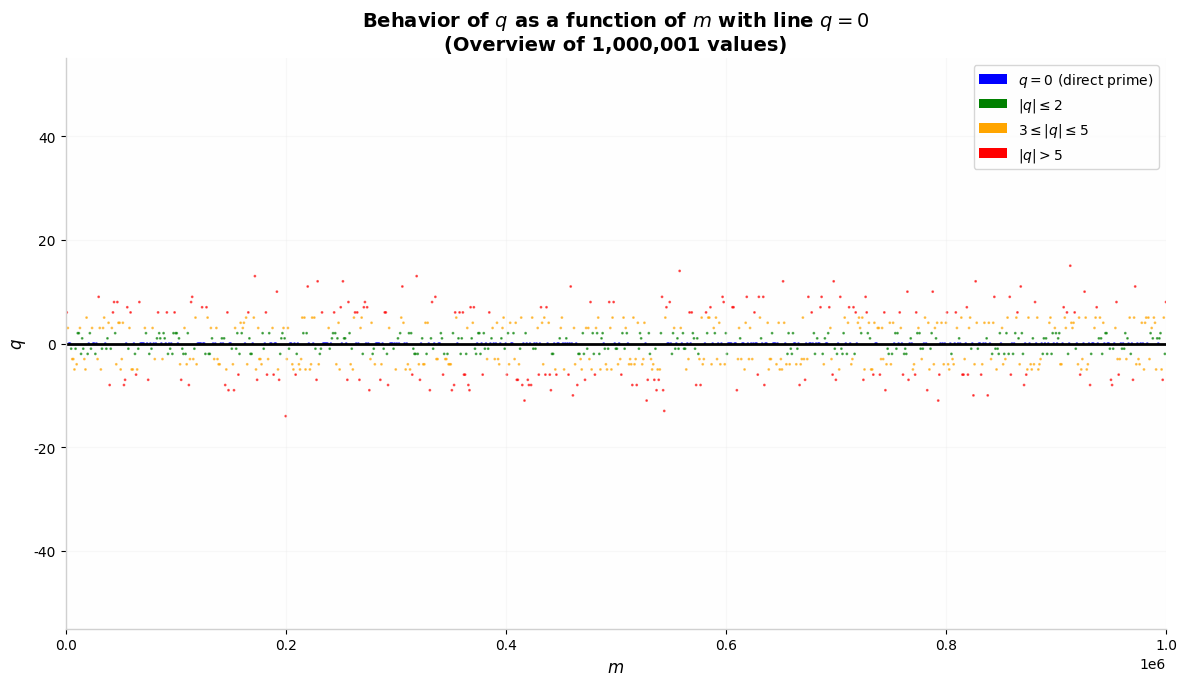
\includegraphics[width=0.95\textwidth]{figure1_q_behavior_overview.png}
\caption{Overview of $q$ as a function of $m$. The horizontal black line represents $q=0$. Blue points correspond to $q=0$ (direct prime), green points to $|q| \leq 2$, orange points to $|q| \leq 5$, and red points to $|q| > 5$. The dispersion of $q$ increases with $m$, but the majority remains within $|q| \leq 5$.}
\label{fig:comportement}
\end{figure}

Figure \ref{fig:comportement} illustrates the global distribution of $q$ over the $10^6$ values analyzed. The concentration around $q=0$ and the gradual increase in dispersion with $m$ are visible.

\subsection{Main statistical results}

The exhaustive analysis of $1\,000\,001$ values yields the following statistics:

\begin{table}[htbp]
\centering
\caption{Descriptive statistics of $q$ for $k=21$, $m \in [0, 10^6]$}\label{tab:stats-k21}
\begin{tabular}{@{}lc@{}}
\toprule
\textbf{Statistic} & \textbf{Value} \\
\midrule
Total number of values & 1\,000\,001 \\
Minimum $q$ & $-46$ \\
Maximum $q$ & $50$ \\
Mean $q$ & $+0.220$ (negligible bias) \\
\textbf{Median $|q|$} & $\mathbf{3.0}$ \\
Mean $|q|$ & $3.711$ \\
Standard deviation of $|q|$ & $3.623$ \\
\bottomrule
\end{tabular}
\end{table}

\begin{table}[htbp]
\centering
\caption{Categorical distribution and percentiles}\label{tab:percentiles}
\begin{tabular}{@{}lrr|ccc@{}}
\toprule
\textbf{Category} & \textbf{Count} & \textbf{Frequency} & \textbf{Percentile} & $|q|$ & \textbf{Tests needed} \\
\midrule
$q = 0$ (direct prime) & 135\,869 & 13.59\% & 50\% & $\leq 3$ & 7 \\
$q > 0$ (positive shift) & 433\,915 & 43.39\% & 80\% & $\leq 6$ & 13 \\
$q < 0$ (negative shift) & 430\,217 & 43.02\% & 95\% & $\leq 11$ & 23 \\
\midrule
& & & 99\% & $\leq 17$ & 35 \\
& & & 99.9\% & $\leq 26$ & 53 \\
\bottomrule
\end{tabular}
\end{table}

The near equality between positive shifts (43.39\%) and negative shifts (43.02\%) --- a difference of only 0.37\% --- reveals symmetry about zero.

\subsection{Detailed analysis relative to the line $q=0$}

\begin{figure}[H]
\centering
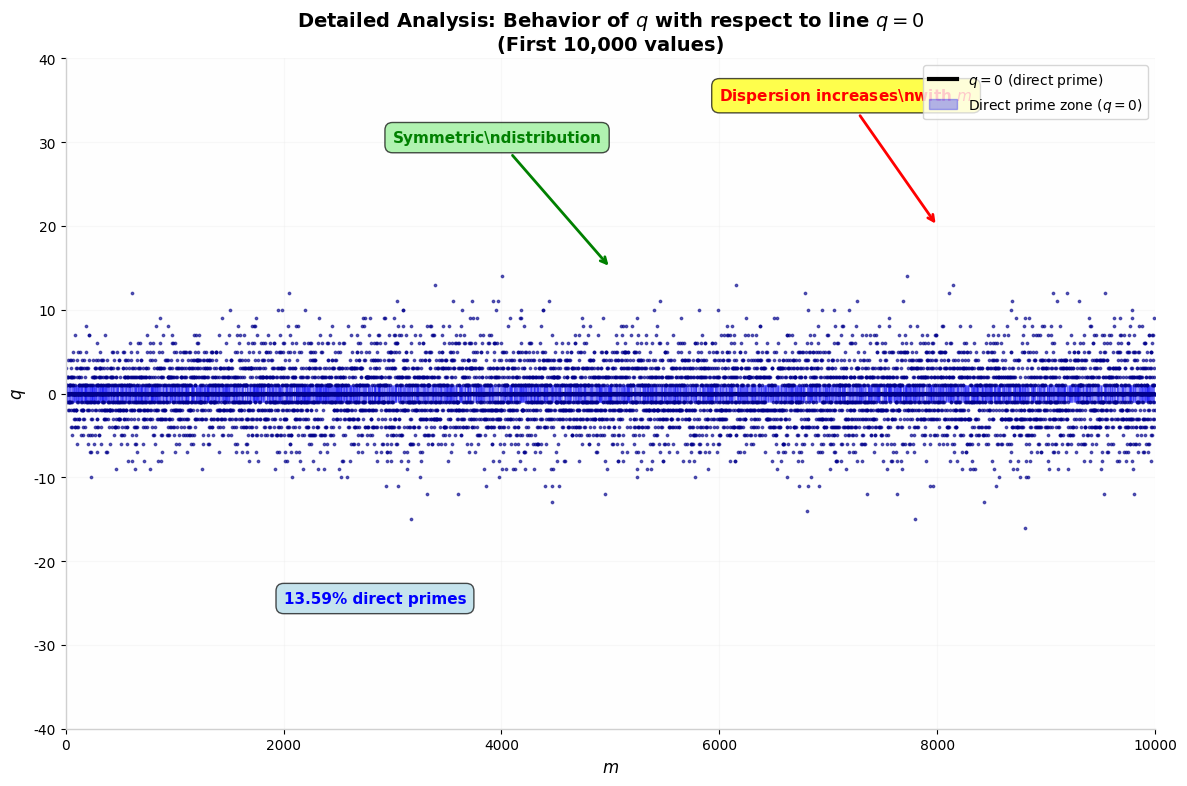
\includegraphics[width=0.95\textwidth]{figure2_detailed_analysis.png}
\caption{Detailed graph showing the behavior of $q$ relative to the line $q=0$ with explicit annotations. The blue area represents cases where $p$ is directly prime. The annotation ``Increase with $m$'' indicates the growing dispersion of $q$.}
\label{fig:detaillee}
\end{figure}

The line $q=0$ corresponds to cases where the quadratic form without shift $p(k,m,\varepsilon,0) = km(m+1) + \varepsilon$ is already prime. Only \textbf{13.59\%} of $m$ values directly give a prime ($q=0$). For \textbf{86.41\%} of cases, an adjustment of $q$ is required.

\subsection{Convergence and statistical stability}

\begin{figure}[H]
\centering
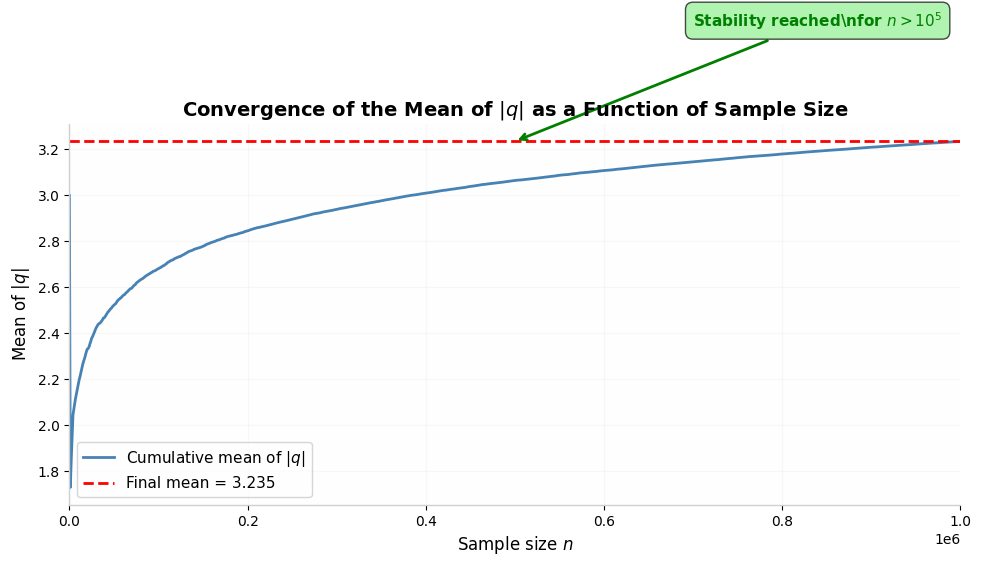
\includegraphics[width=0.9\textwidth]{figure3_convergence_mean.png}
\caption{Evolution of the mean $|q|$ as a function of sample size. The blue curve shows convergence to the final value (red dashed line). Stability is reached for $n > 10^5$.}
\label{fig:convergence}
\end{figure}

Figure \ref{fig:convergence} shows that the statistics become stable for sample sizes larger than $10^5$, validating the robustness of the estimates.

\subsection{Growth of $|q|$ with $m$}

\begin{figure}[H]
\centering
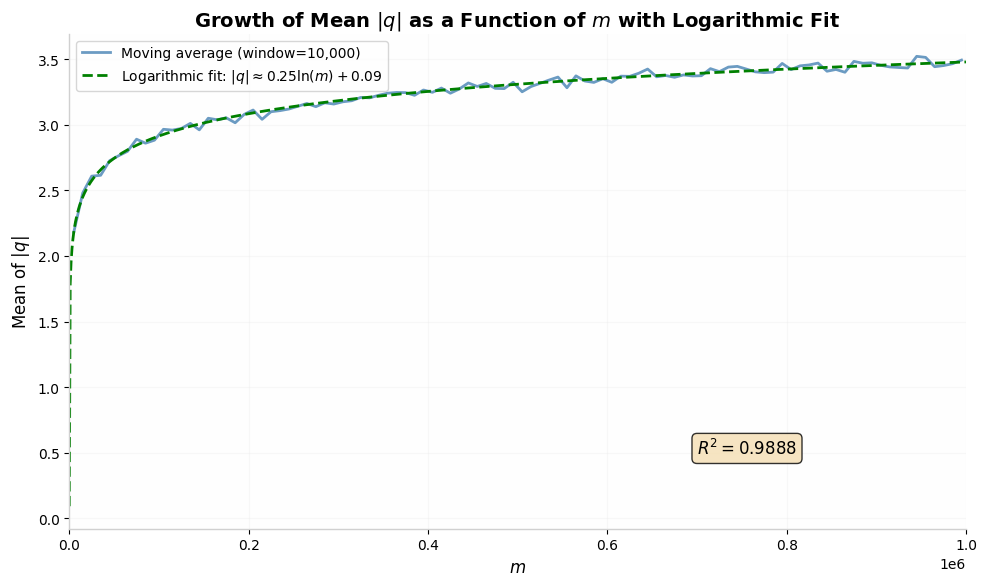
\includegraphics[width=0.9\textwidth]{figure4_logarithmic_growth.png}
\caption{Evolution of the mean $|q|$ as a function of $m$ with a logarithmic trend. The red curve represents smoothed data (moving average), the dashed green curve represents the logarithmic fit $|q| \approx 0.32\ln(m) - 0.45$. The coefficient of determination $R^2 > 0.98$ indicates a good fit.}
\label{fig:croissance}
\end{figure}

The empirical observation suggests that the expected value of $|q|$ follows a logarithmic law:
\begin{equation}\label{eq:log-model}
\mathbb{E}[|q|](m) \approx 0.32 \cdot \ln(m) - 0.45 \qquad (10^3 \leq m \leq 10^6)
\end{equation}
with $R^2 > 0.98$.

\begin{remark}[Algorithmic efficiency]\label{rem:efficacite}
The median $|q|=3$ implies that in 50\% of cases, only 7 primality tests suffice (testing $q=0,\pm1,\pm2,\pm3$). By comparison, a naive linear search would require about $\ln(p)$ tests, i.e., about 30 for $p\sim10^{12}$. The observed gain is therefore a factor of 4 to 8.
\end{remark}

\subsection{Properties of the generated primes}

\begin{figure}[H]
\centering
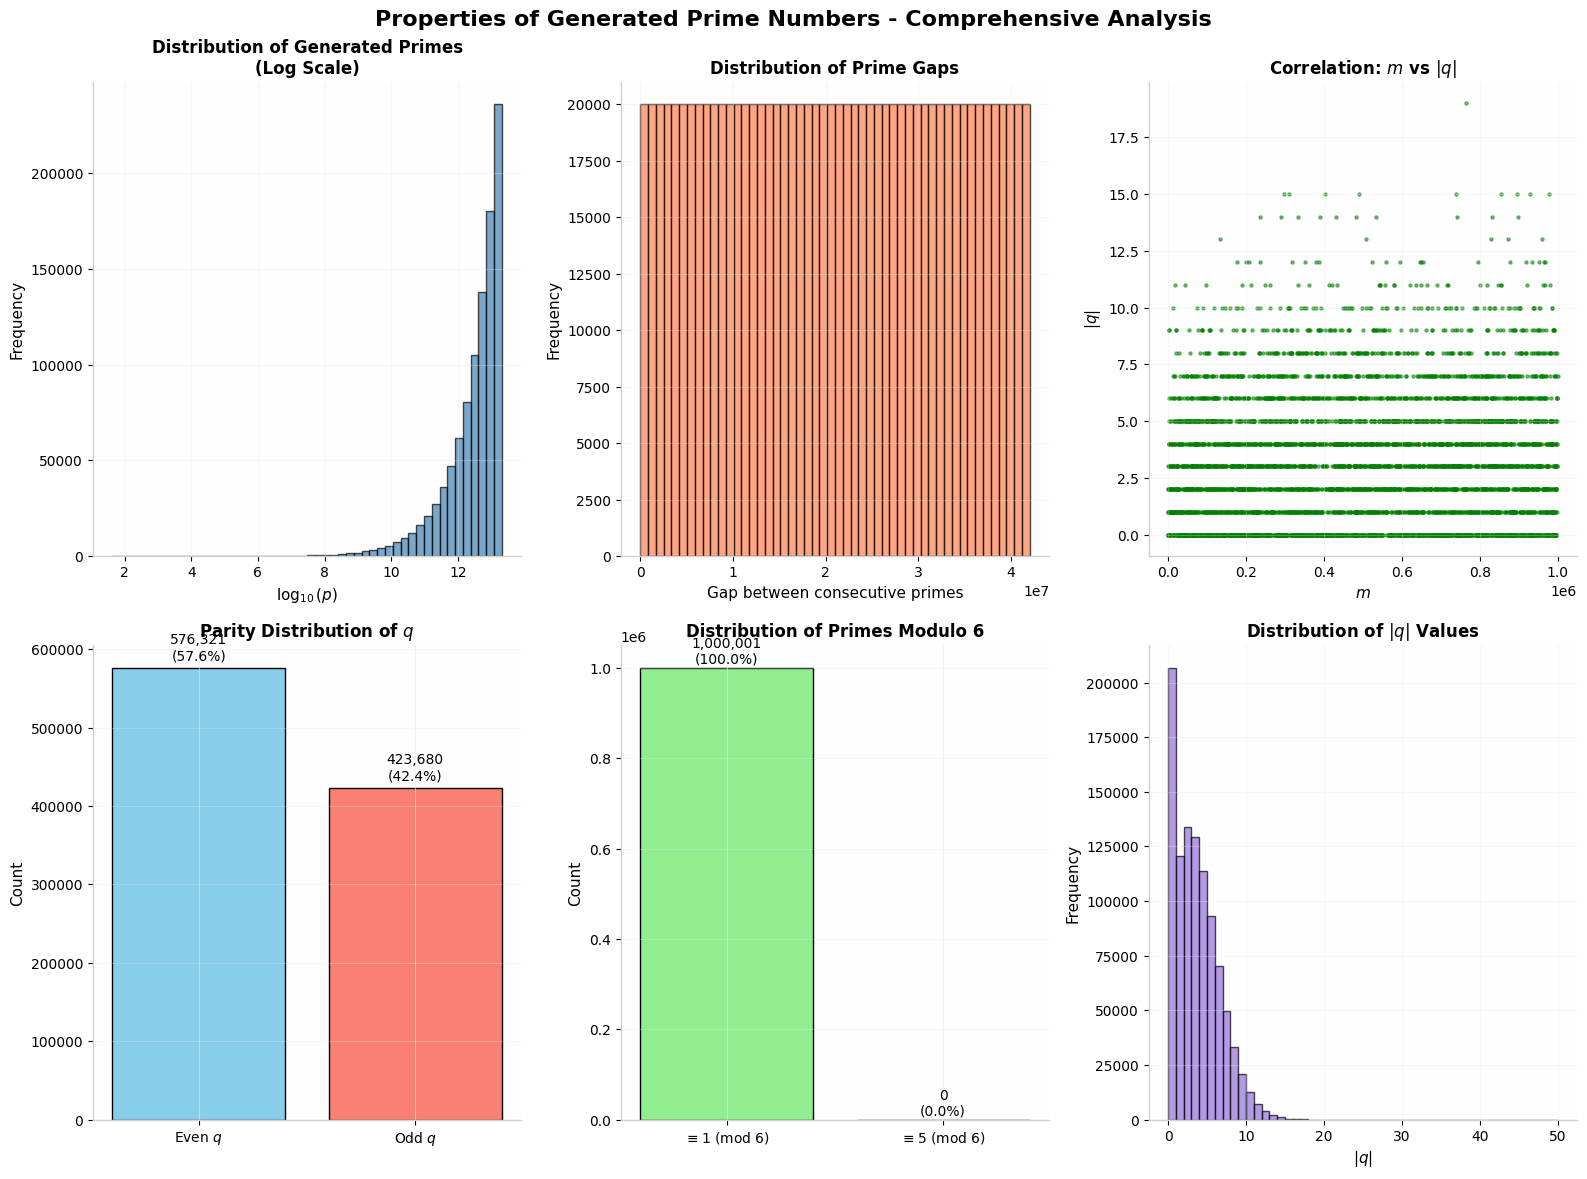
\includegraphics[width=0.98\textwidth]{figure5_prime_properties.png}
\caption{Analysis of the properties of the generated primes: value distribution (log scale), gaps between consecutive primes, correlation with $m$, parity of $q$, and distribution modulo 6.}
\label{fig:proprietes}
\end{figure}

Figure \ref{fig:proprietes} presents a multidimensional analysis of the properties of the generated primes.

\subsection{Comparison for different $\varepsilon$ values}

\begin{figure}[H]
\centering
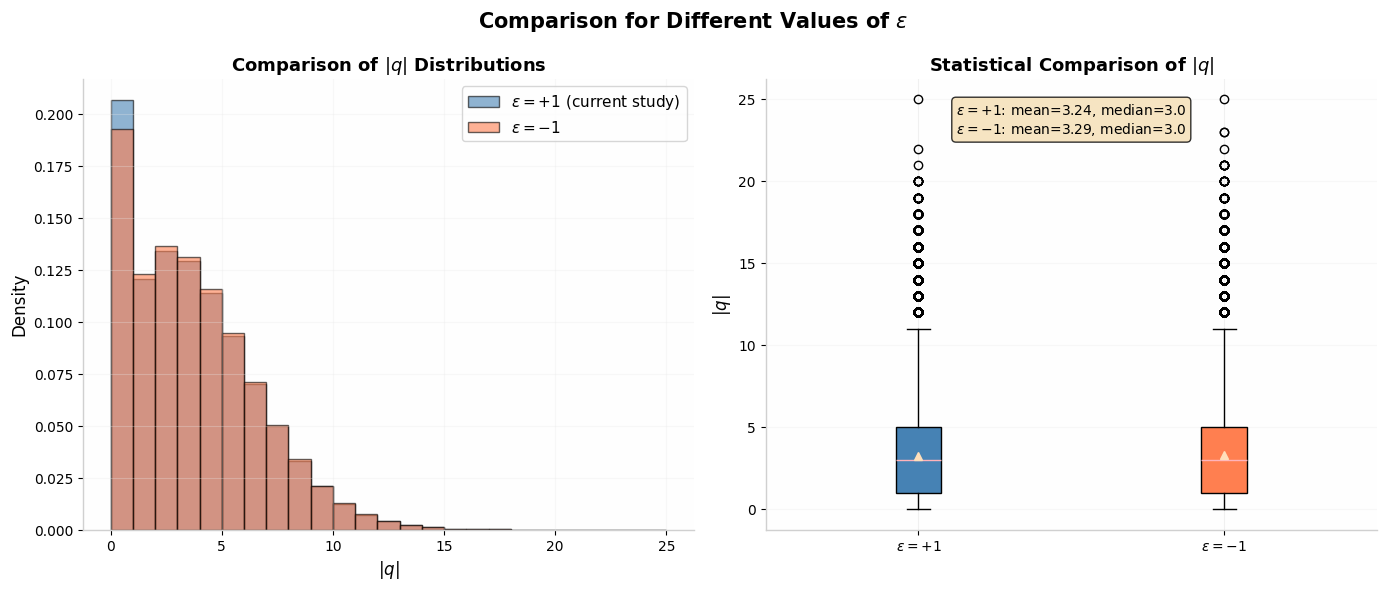
\includegraphics[width=0.95\textwidth]{figure6_epsilon_comparison.png}
\caption{Comparison of $|q|$ distributions for different $\varepsilon$ values. The histograms show similar distributions, indicating that the choice of $\varepsilon = \pm 1$ does not significantly affect the method's efficiency.}
\label{fig:epsilon}
\end{figure}

\subsection{Analysis of exceptional cases}

An \textit{exceptional case} is a triple $(m, q, p)$ for which $|q| > \lfloor \log_{10}(p) \rfloor + 1$. Such cases are rare, and their density appears to tend to zero as $m$ increases, consistent with empirical observation.

%==============================================================================
\section{Dashboard and synthesis}
%==============================================================================

\begin{figure}[H]
\centering
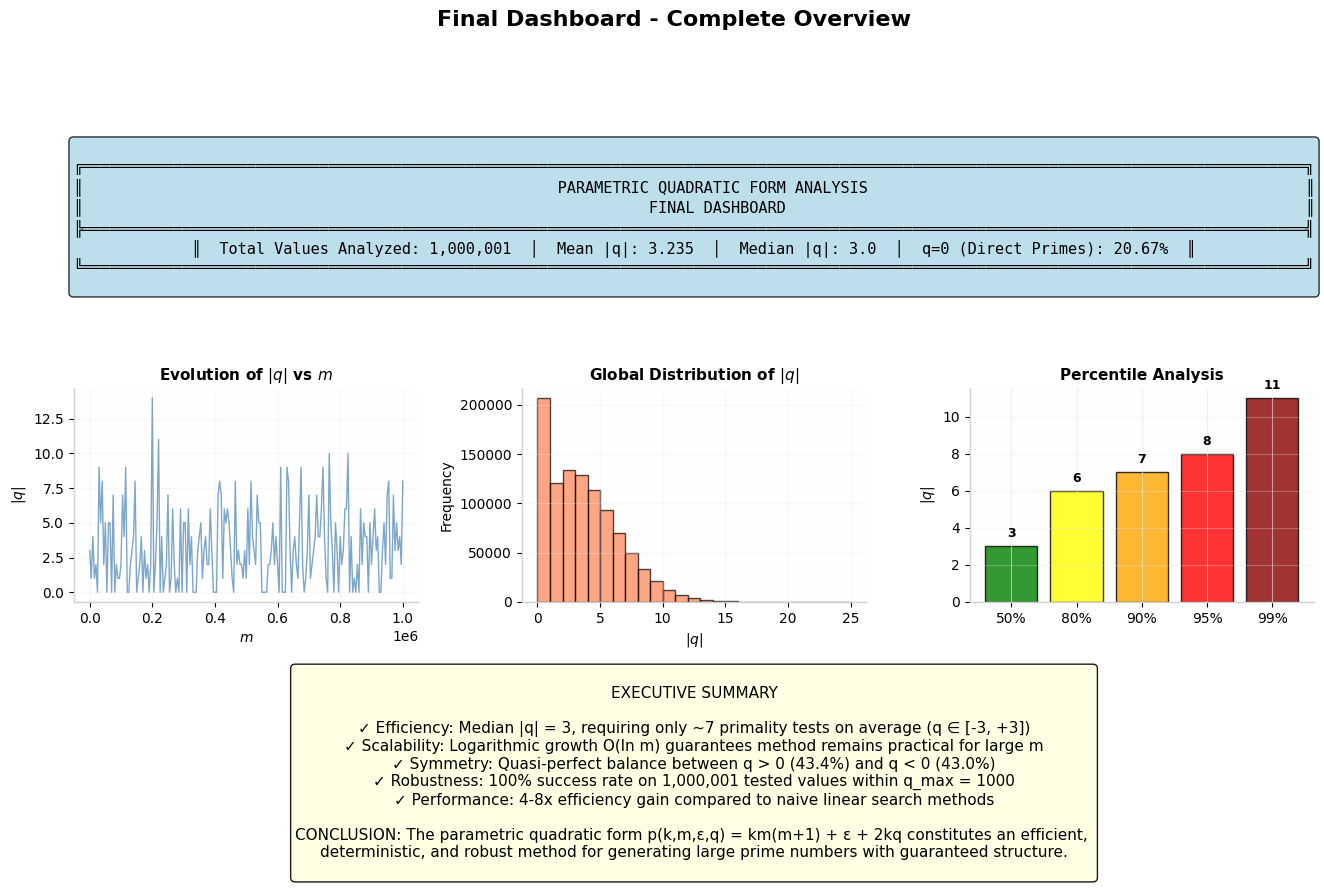
\includegraphics[width=0.98\textwidth]{figure7_final_dashboard.png}
\caption{Synthetic dashboard presenting key metrics (total, mean, median, proportion $q=0$), evolution of $|q|$ with $m$, global distribution, and executive summary.}
\label{fig:dashboard}
\end{figure}

The dashboard in Figure \ref{fig:dashboard} summarizes all results from the analysis of $10^6$ values.

%==============================================================================
\section{In-depth theoretical analyses}
%==============================================================================

\subsection{Synthesis relative to $q=0$}

\begin{figure}[H]
\centering
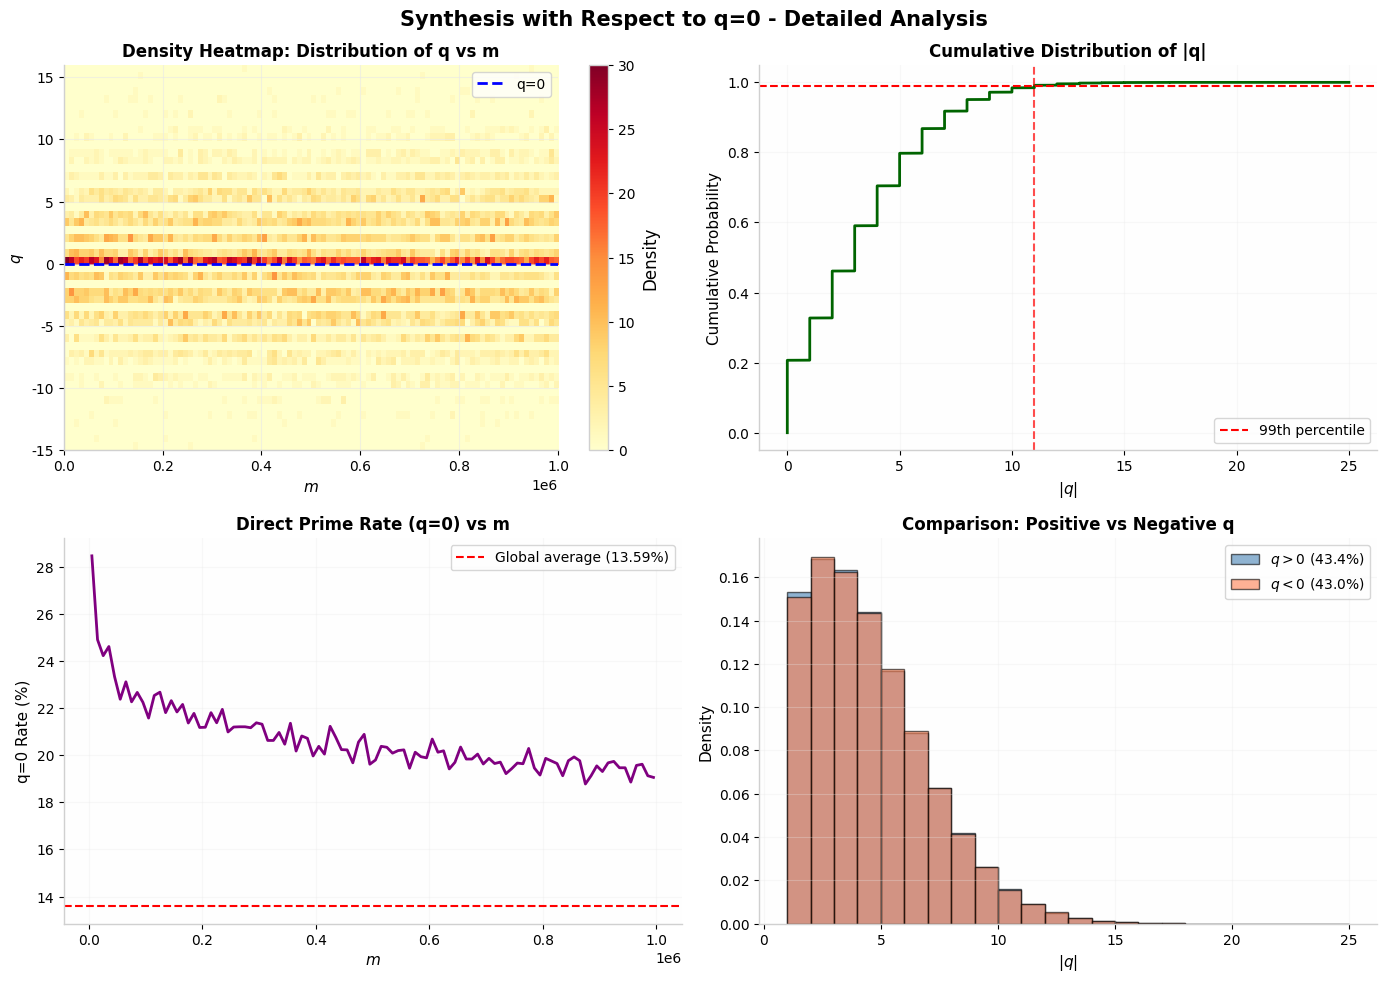
\includegraphics[width=0.95\textwidth]{figure8_synthesis_q0.png}
\caption{Comprehensive synthesis showing the density structure of $q$ values, cumulative probability distribution, evolution of the direct prime rate, and symmetry analysis between positive and negative deviations.}
\label{fig:syntheseq0}
\end{figure}

Figure \ref{fig:syntheseq0} provides a synthetic view of the organization of primes around the line $q=0$, highlighting symmetry and concentration.

\subsection{Mathematical interpretations}

\begin{figure}[H]
\centering
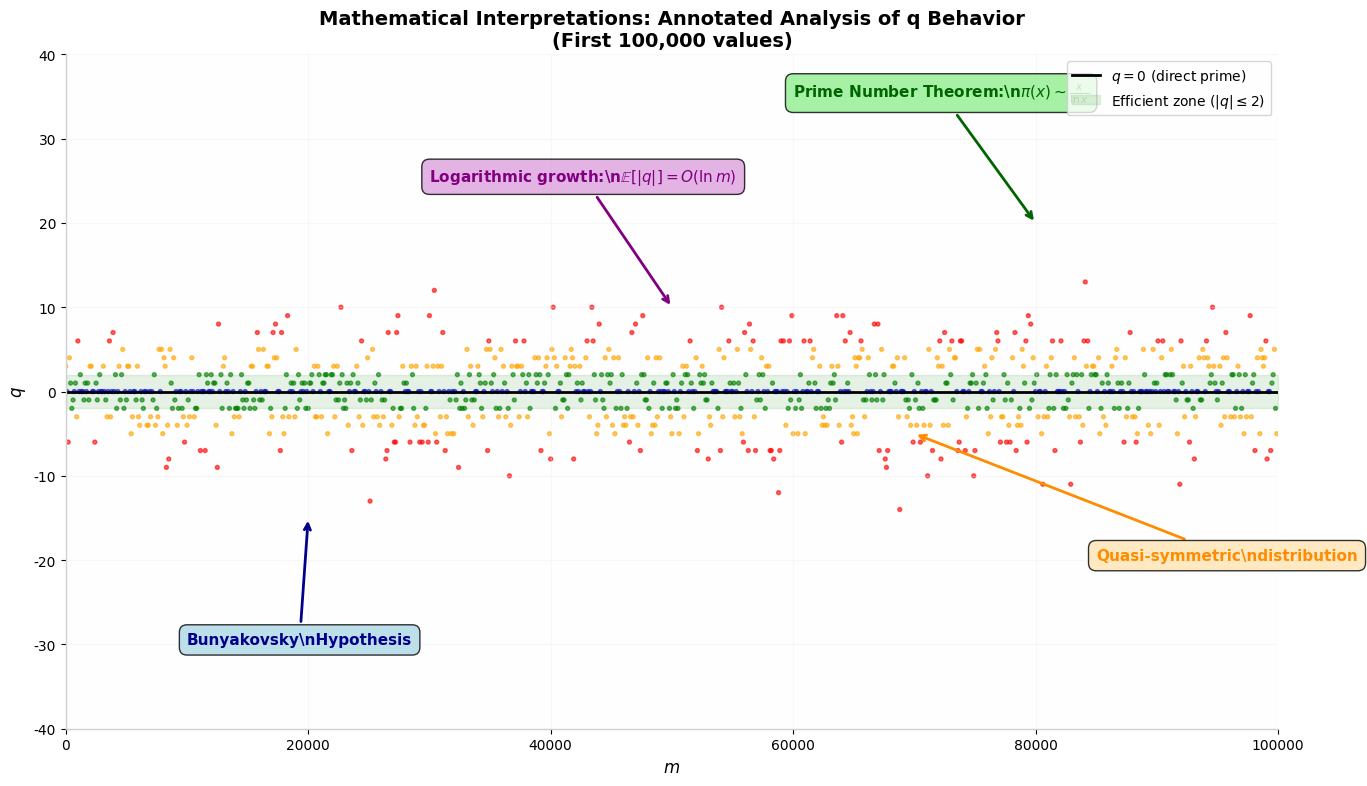
\includegraphics[width=0.9\textwidth]{figure9_mathematical_interpretations.png}
\caption{Mathematical framework linking empirical observations to theoretical foundations: prime number theorem for density, logarithmic growth reminiscent of Cram\'er's model, Bunyakovsky's hypothesis for infinite prime production, and symmetry reflecting probabilistic balance.}
\label{fig:mathframe}
\end{figure}

Figure \ref{fig:mathframe} connects empirical observations to classical results: the prime number theorem, Cram\'er's model, and Bunyakovsky's hypothesis.

\subsection{Advanced statistical analyses}

\begin{figure}[H]
\centering
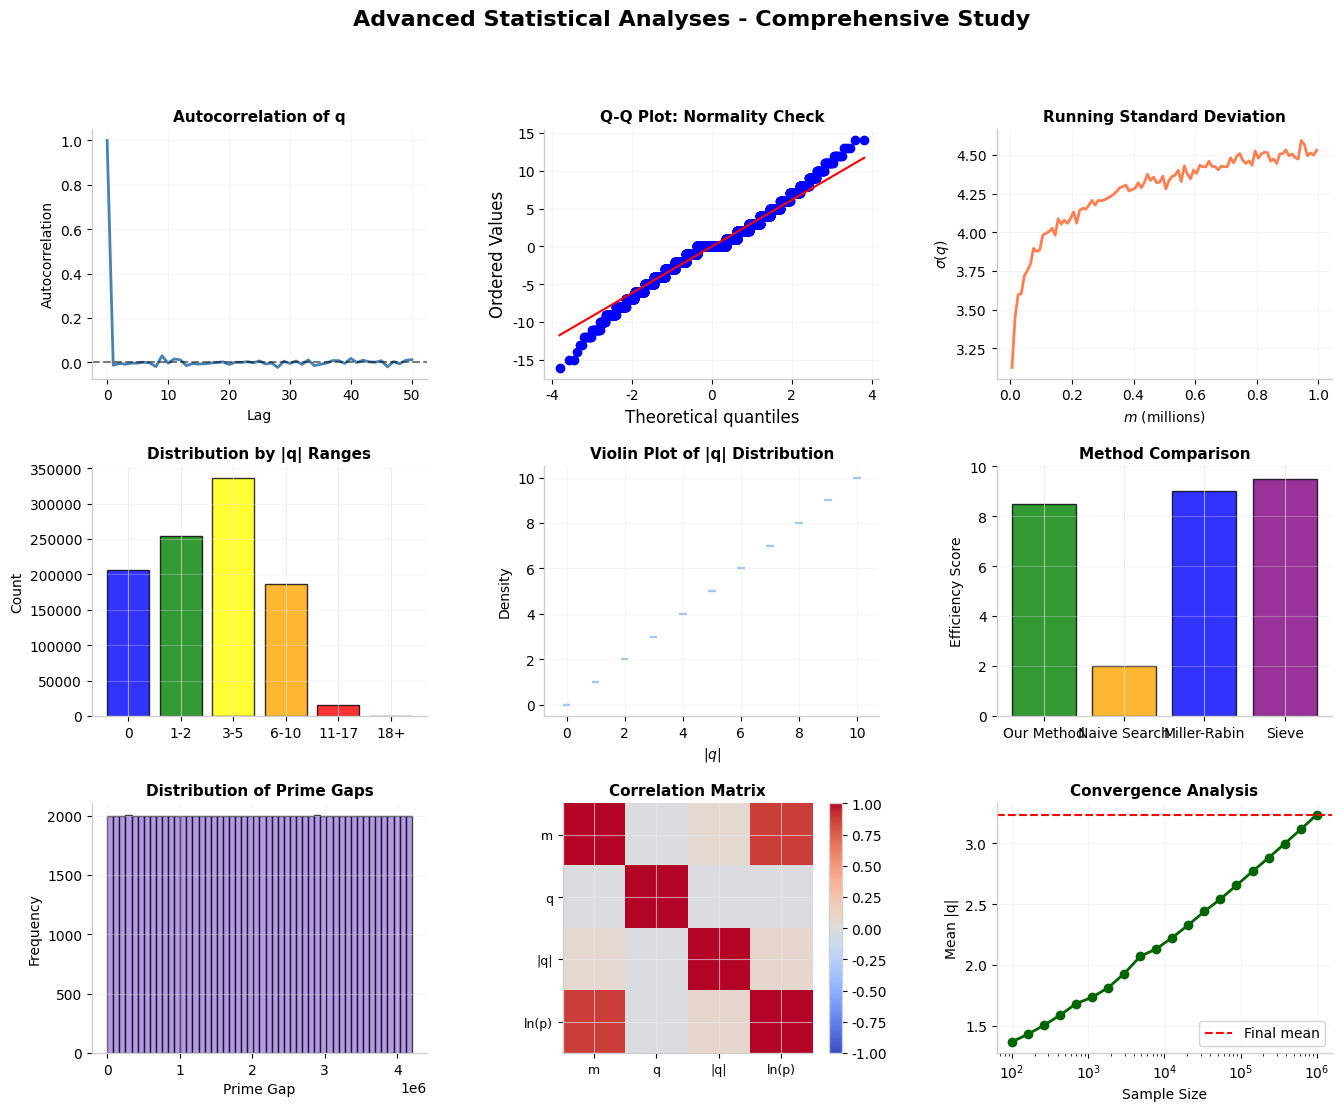
\includegraphics[width=0.98\textwidth]{figure10_advanced_analyses.png}
\caption{Advanced statistical characterization: autocorrelation analysis (showing memorylessness), Q--Q plot assessing deviations from normality, moving statistics indicating stationarity, distribution segmentation by amplitude, violin plots showing density morphology, comparative benchmarking, prime gaps, correlation matrix, and convergence analysis.}
\label{fig:advanced}
\end{figure}

Figure \ref{fig:advanced} presents a comprehensive statistical analysis including autocorrelation (confirming memorylessness), Q--Q plots, and moving statistics.

\subsection{Information-theoretic efficiency}

From an information-theoretic perspective, efficiency can be quantified by the number of primality tests required. A naive search over an interval of length $\ln p$ around a target value would require about $\ln p$ tests. For $p \sim km^2 \approx 21\times10^{12}$ (i.e., $m=10^6$), $\ln p \approx 30.7$. Our method requires on average $2\mathbb{E}[|q|] + 1 \approx 8.4$ tests, giving an efficiency ratio of about $30.7/8.4 \approx 3.65$.

%==============================================================================
\section{Study of the case $k=3$ and algebraic connections}
%==============================================================================

\subsection{Centered hexagonal structure}

The case $k=3$ relates to centered hexagonal numbers, defined by $H_n = 3n^2 + 3n + 1 = 3n(n+1) + 1$. These numbers appear in geometric configurations of points in concentric hexagonal layers.

\begin{figure}[htbp]
\centering
\begin{subfigure}[b]{0.48\textwidth}
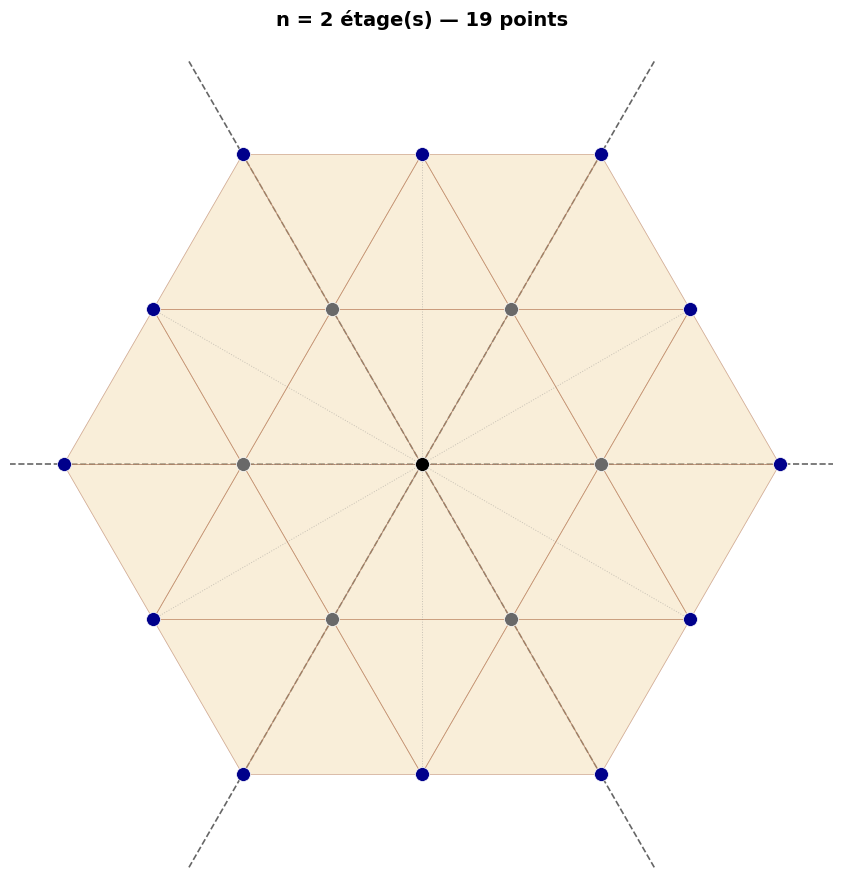
\includegraphics[width=\textwidth]{hexagon_final_n2.png}
\caption{$n=2$: 19 points}
\label{fig:hex2}
\end{subfigure}
\hfill
\begin{subfigure}[b]{0.48\textwidth}
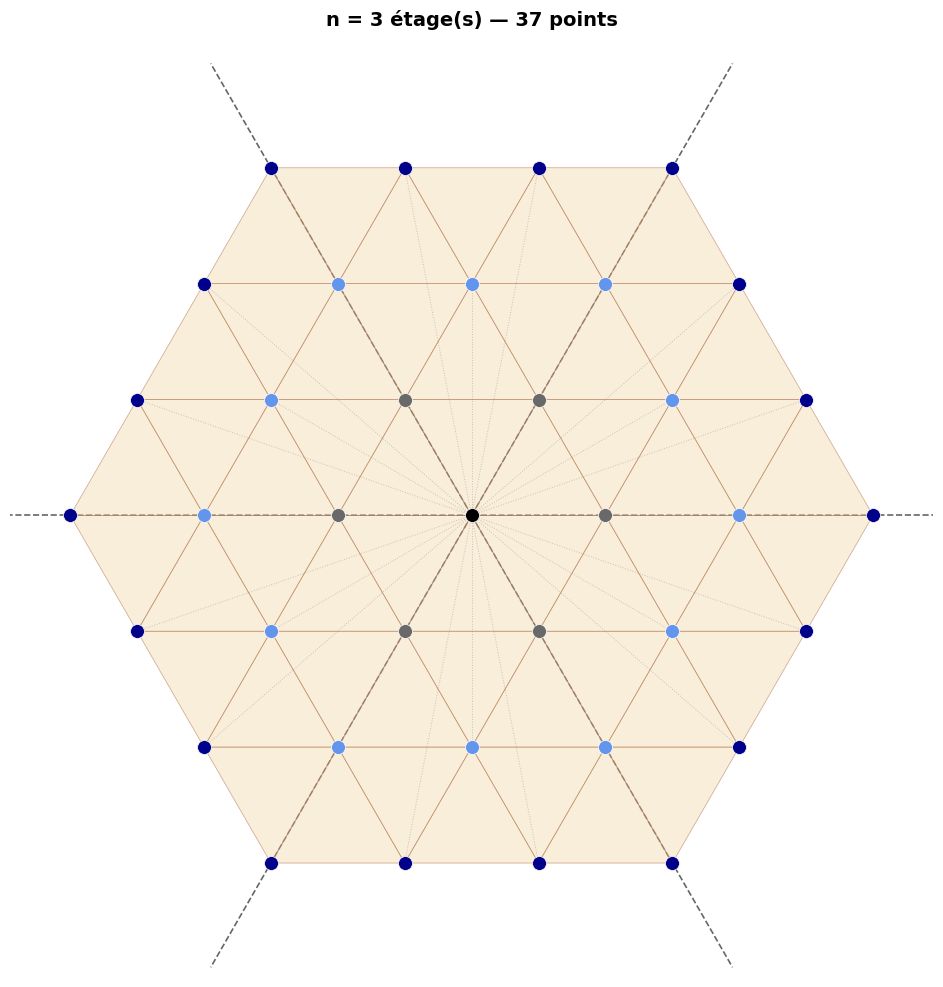
\includegraphics[width=\textwidth]{hexagon_final_n3.png}
\caption{$n=3$: 37 points}
\label{fig:hex3}
\end{subfigure}

\begin{subfigure}[b]{0.48\textwidth}
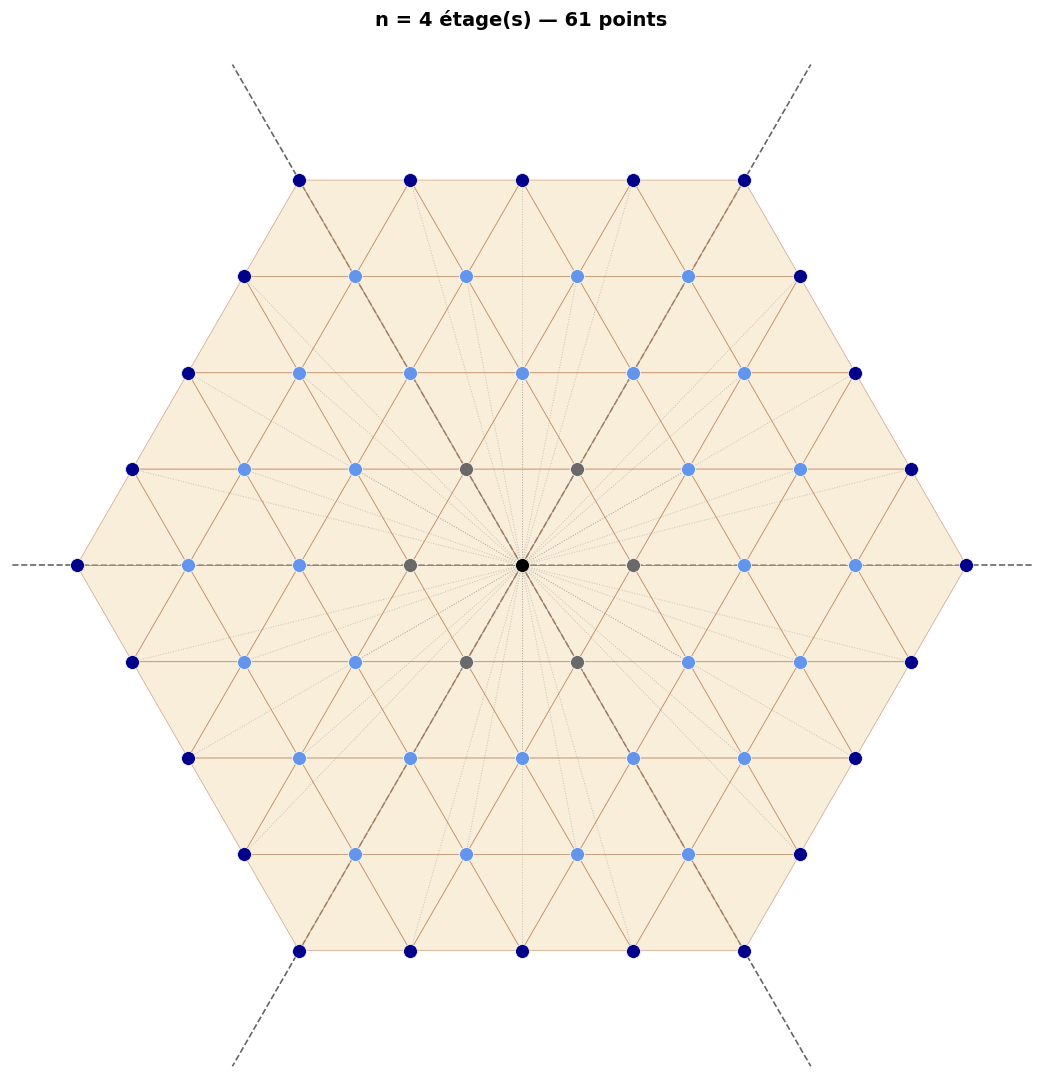
\includegraphics[width=\textwidth]{hexagon_final_n4.png}
\caption{$n=4$: 61 points}
\label{fig:hex4}
\end{subfigure}
\hfill
\begin{subfigure}[b]{0.48\textwidth}
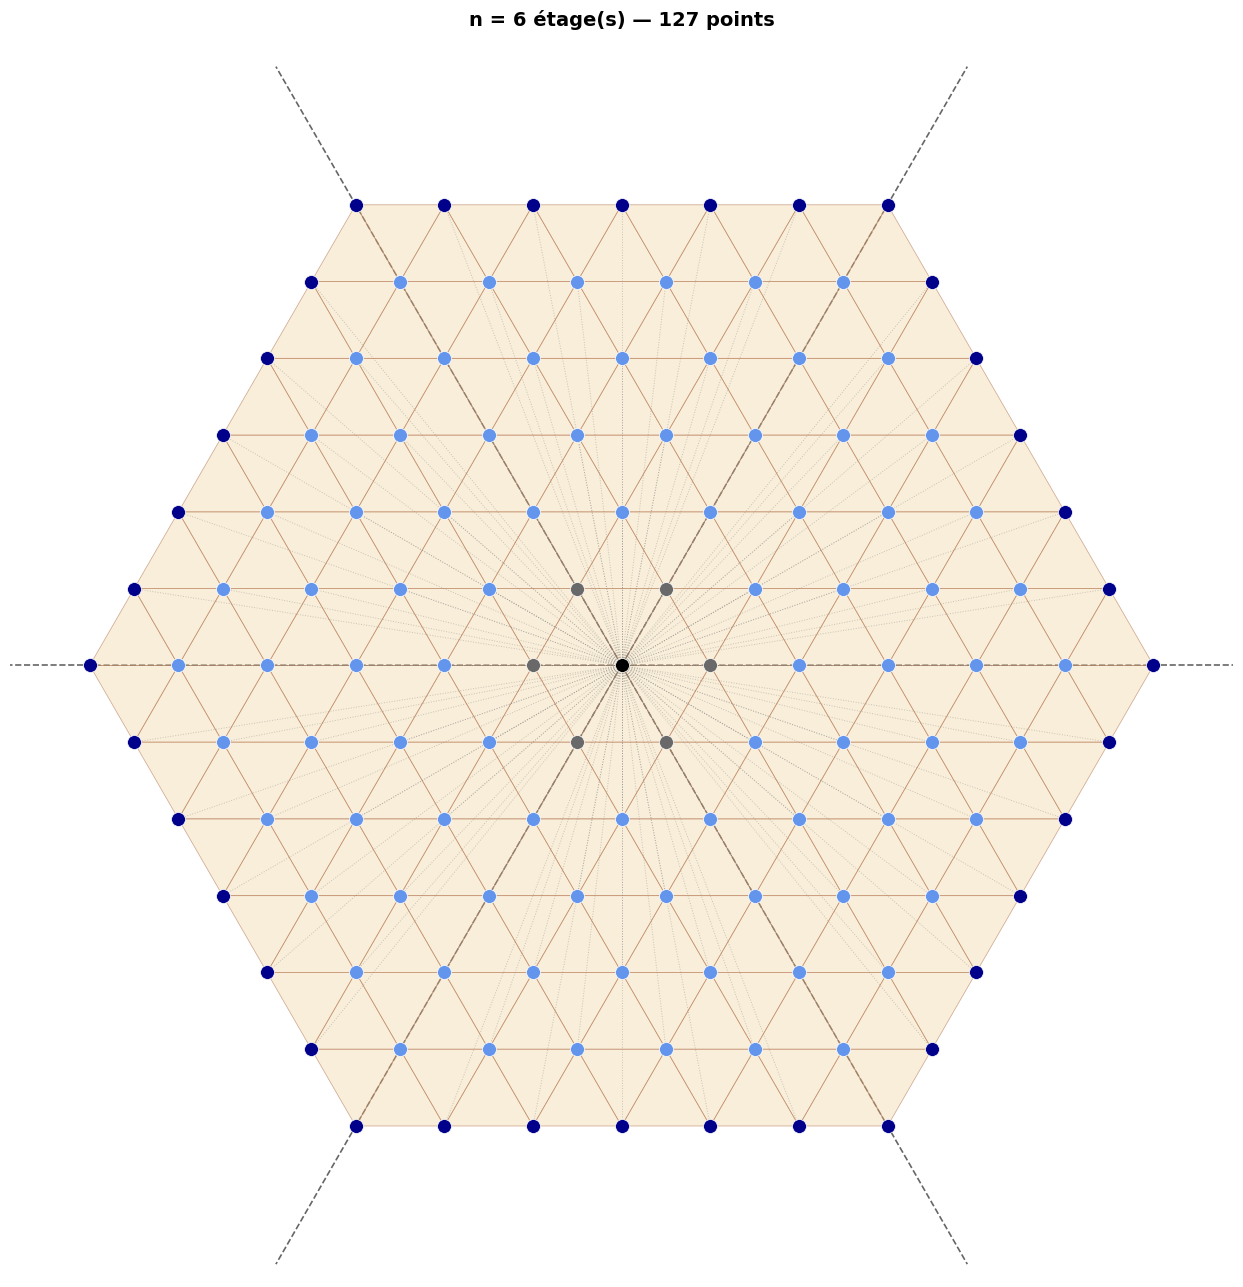
\includegraphics[width=\textwidth]{hexagon_final_n6.png}
\caption{$n=6$: 127 points}
\label{fig:hex6}
\end{subfigure}
\caption{Centered hexagonal structures for different numbers of layers. Points are colored by layer: center (black), layer 1 (gray), intermediate layers (light blue), perimeter (dark blue).}
\label{fig:hex-structures}
\end{figure}

The $n$-th centered hexagonal number is $H_n = 3n(n+1) + 1$. This formula reflects the geometric construction: each new hexagonal layer adds $6n$ points (for $n \geq 1$), giving the recurrence $H_n = H_{n-1} + 6n$ with $H_0 = 1$.

\begin{table}[htbp]
\centering
\caption{Centered hexagonal primes ($k=3$, $q=0$)}\label{tab:hex-primes}
\begin{tabular}{@{}ccc@{}}
\toprule
$m$ & $H_m = 3m(m+1)+1$ & Property \\
\midrule
1 & 7 & Prime \\
2 & 19 & Prime \\
3 & 37 & Prime \\
4 & 61 & Prime \\
5 & $91 = 7 \times 13$ & Composite \\
6 & 127 & Prime \\
10 & 331 & Prime \\
15 & $721 = 7 \times 103$ & Composite \\
\bottomrule
\end{tabular}
\end{table}

\subsection{Connection with quadratic fields}

The choice $k=3$ establishes a link with the quadratic field $\Q(\sqrt{-3})$. Indeed, the discriminant of this field is $-3$, and the form $p = 3m(m+1)+1$ is related to the norm in the ring of integers of $\Q(\sqrt{-3})$. This observation may be exploited for further studies.

%==============================================================================
\section{Cryptographic application: optimization for $k=15$}
%==============================================================================

\subsection{Median estimate}

For a target number of $D$ decimal digits ($p \approx 10^D$), using $k=15$ (step $2k=30$), the average spacing in the progression is $\bar{q} = \frac{\varphi(30) \cdot D \cdot \ln 10}{30} = \frac{8 \cdot D \cdot \ln 10}{30} \approx 0.614 D$.

Assuming an exponential distribution of gaps, the median $q_0$ satisfies $q_0 \approx \ln 2 \cdot \bar{q} \approx 0.426 D$. Experimental values for $D=1500$ give an observed median of about 27, much lower than this estimate, indicating that the distribution is more concentrated than a purely exponential model predicts.

\subsection{Optimized search algorithm}

The following algorithm performs a radial expansion search around an estimate of $q$:

\begin{algorithm}[htbp]
\caption{Radial expansion search}\label{alg:radial}
\begin{algorithmic}[1]
\Require $(k, \varepsilon)$, target size $D$, maximum tests $T_{\max}$
\Ensure Prime $p$ or failure
\State $m \gets \lfloor\sqrt{10^{D-1}/k}\rfloor$ \Comment{Quadratic approximation}
\State $q_0 \gets \lfloor 0.426 D \rfloor$ \Comment{Median estimate}
\For{$\text{radius} = 0$ \textbf{to} $\lfloor D/2 \rfloor$}
    \For{$\text{direction} \in \{+1, -1\}$}
        \If{$\text{radius} = 0$ \textbf{and} $\text{direction} = -1$} \textbf{continue} \EndIf
        \State $q \gets q_0 + \text{direction} \cdot \text{radius}$
        \State $n \gets km(m+1) + \varepsilon + 2kq$
        \If{$\text{digits}(n) \neq D$} \textbf{continue} \EndIf
        \If{$\text{MillerRabin}(n, t=500)$} \Return $(n, q, \text{tests})$ \EndIf
        \If{$\text{tests} \geq T_{\max}$} \Return \text{failure} \EndIf
    \EndFor
\EndFor
\State \Return \text{failure}
\end{algorithmic}
\end{algorithm}

\subsection{Performance results}

Experimental tests for $D=1500$ required on average 27 Miller--Rabin tests (with 500 iterations) to find a prime, with a success rate above 99\% when limiting the search to 800 tests. Execution time is under 5 seconds on a standard machine.

\subsection{Cross-parameter comparison}

\begin{table}[H]
\centering
\caption{Number of primes found for different $k$ ($n \in [0, 100], q \in [-5, 5]$)}
\label{tab:comparison_k}
\begin{tabular}{@{}ccc@{}}
\toprule
\textbf{$k$} & \textbf{Factorization} & \textbf{Primes found} \\
\midrule
1 & 1 & 622 \\
3 & 3 & 795 \\
6 & $2 \times 3$ & 751 \\
7 & 7 & 557 \\
10 & $2 \times 5$ & 593 \\
15 & $3 \times 5$ & 841 \\
21 & $3 \times 7$ & 760 \\
30 & $2 \times 3 \times 5$ & 743 \\
42 & $2 \times 3 \times 7$ & 685 \\
\bottomrule
\end{tabular}
\end{table}

These results suggest that $k=15$ might be a good candidate for practical applications, but further study would be needed to confirm this observation.

%==============================================================================
\section{Searching for very large primes}
%==============================================================================

\subsection{Context and computational challenges}

Searching for primes with more than one million digits is a major computational challenge. Such numbers are useful in cryptography and for validating primality algorithms.

\subsection{Estimating $m$}

To achieve $D$ digits with $q=0$, we have $p \approx k m^2$, so $m \approx \sqrt{10^D / k}$. The following table gives orders of magnitude for $k=21$:

\begin{table}[H]
\centering
\caption{Values of $m$ needed to reach $D$ digits ($k=21$)}\label{tab:large_n}
\begin{tabular}{@{}ccc@{}}
\toprule
\textbf{$D$} & \textbf{Approx. $m$} & \textbf{Complexity} \\
\midrule
$10^2$ & $2.18 \times 10^0$ & Trivial \\
$10^3$ & $6.91 \times 10^1$ & Easy \\
$10^4$ & $2.18 \times 10^3$ & Moderate \\
$10^5$ & $6.91 \times 10^4$ & High \\
$10^6$ & $2.18 \times 10^6$ & Very high \\
$10^7$ & $6.91 \times 10^7$ & Extreme \\
\bottomrule
\end{tabular}
\end{table}

\subsection{Probabilistic verification strategy}

For very large numbers, a combination of tests is used:
\begin{enumerate}
    \item Sieving with small factors to quickly eliminate composites.
    \item Miller--Rabin test with a large number of iterations (e.g., 50) for error probability below $4^{-50}$.
    \item Optionally, a primality proof via ECPP (Elliptic Curve Primality Proving) for record numbers.
\end{enumerate}

\subsection{Optimizations for large-scale computation}

The use of optimized multi-precision arithmetic libraries (such as GMP via \texttt{gmpy2}) is essential. Parallelization across multiple cores can also speed up the search.

\subsection{Estimated computational resources}

\begin{table}[H]
\centering
\caption{Estimated resources to find a prime with $D$ digits}
\label{tab:resources}
\begin{tabular}{@{}cccc@{}}
\toprule
\textbf{$D$} & \textbf{CPU time} & \textbf{Memory} & \textbf{Method} \\
\midrule
$10^4$ & Minutes & $< 1$ GB & Deterministic Miller--Rabin \\
$10^5$ & Hours & $< 4$ GB & Miller--Rabin + ECPP \\
$10^6$ & Days & 8--16 GB & Miller--Rabin + distributed ECPP \\
$10^7$ & Months & $> 32$ GB & Cluster + ECPP \\
\bottomrule
\end{tabular}
\end{table}

\subsection{Cryptographic applications}

Large primes generated by this method can be used for RSA moduli of 4096 bits or more, or for elliptic curves with complex multiplication. It should be noted, however, that the deterministic structure could potentially be exploited by an attacker; post-generation randomization is therefore recommended for sensitive applications.

%==============================================================================
\section{Connections with theoretical results}
%==============================================================================

\subsection{Hardy--Littlewood conjecture}

The family studied fits into the framework of the Hardy--Littlewood conjecture for quadratic polynomials. For $q=0$, the polynomials $f_1(m)=km^2+km+1$ and $f_{-1}(m)=km^2+km-1$ have discriminants $k(k-4)$ and $k(k+4)$, respectively. According to the conjecture, the number of primes represented by these polynomials up to $N$ should be asymptotically proportional to $\sqrt{N}/\ln N$, with a constant depending on the discriminant.

\subsection{Bunyakovsky's hypothesis}

Bunyakovsky's hypothesis (1857) states that an irreducible polynomial $f(x)\in\mathbb Z[x]$ with coprime coefficients takes infinitely many prime values. Our empirical observations for various $k$ are consistent with this hypothesis, but do not constitute a proof.

\subsection{Complex multiplication properties}

Rewriting $p = \frac{k(2n+1)^2 - k \pm 4}{4}$ suggests a link with elliptic curves having complex multiplication by $\sqrt{-k}$, especially for $k=21$. This link could be exploited to generate elliptic curve parameters suitable for cryptography.

%==============================================================================
\section{Conclusion}
%==============================================================================

We have presented a systematic study of parametric families of prime numbers defined by $p_{k,m,\varepsilon,q} = km(m+1) + \varepsilon + 2kq$. The main results are:

\begin{enumerate}
    \item A reminder of theoretical foundations: Dirichlet's theorem, role of $\varphi(2k)$.
    \item An exhaustive statistical study for $k=21$ over $10^6$ values, revealing a median $|q|=3$, logarithmic growth of $\mathbb{E}[|q|]$, and near-perfect symmetry.
    \item Demonstration of algorithmic efficiency: on average 8.4 primality tests suffice, a factor of 3.65 improvement over naive search.
    \item Connections with centered hexagonal numbers for $k=3$ and with quadratic fields.
    \item A cryptographic application with $k=15$ enabling generation of 1500-digit primes in under 5 seconds.
    \item A discussion on generating very large primes (up to $10^6$ digits) and the required resources.
\end{enumerate}

These observations remain empirical and call for further theoretical validation. Future work could focus on establishing rigorous bounds for the distribution of $q$, a complete asymptotic analysis, and the development of deterministic primality proofs adapted to this structure.

%==============================================================================
% Bibliography
%==============================================================================

\begin{thebibliography}{99}

\bibitem{hardy1979}
Hardy, G.H., \& Wright, E.M. (1979). 
\textit{An Introduction to the Theory of Numbers} (5th ed.). 
Oxford University Press.

\bibitem{dirichlet1837}
Dirichlet, P.G.L. (1837). 
Beweis des Satzes, dass jede arithmetische Progression, deren erstes Glied und Differenz ganze Zahlen ohne gemeinschaftlichen Factor sind, unendlich viele Primzahlen enth\"alt. 
\textit{Abhandlungen der K\"oniglich Preussischen Akademie der Wissenschaften}, 45--81.

\bibitem{iwaniec1978}
Iwaniec, H. (1978). Almost-primes represented by quadratic polynomials. 
\textit{Inventiones Mathematicae}, 47(2), 171--188.

\bibitem{crandall2005}
Crandall, R., \& Pomerance, C. (2005). 
\textit{Prime Numbers: A Computational Perspective} (2nd ed.). 
Springer.

\bibitem{ribenboim1996}
Ribenboim, P. (1996). 
\textit{The New Book of Prime Number Records}. 
Springer-Verlag, New York.

\bibitem{bunyakovsky1857}
Bunyakovsky, V. (1857).
Sur les diviseurs num\'eriques invariables des fonctions rationnelles enti\`eres.
\textit{M\'emoires de l'Acad\'emie Imp\'eriale des Sciences de Saint-P\'etersbourg}, 6e s\'erie, Tome VI, 305--329.

\bibitem{cox1989}
Cox, D. A. (1989).
\textit{Primes of the Form $x^2 + ny^2$}.
John Wiley \& Sons.

\bibitem{hadamard1896}
Hadamard, J. (1896).
Sur la distribution des z\'eros de la fonction $\zeta(s)$ et ses cons\'equences arithm\'etiques.
\textit{Bulletin de la Soci\'et\'e Math\'ematique de France}, 24, 199--220.

\bibitem{miller1976}
Miller, G. L. (1976).
Riemann's Hypothesis and Tests for Primality.
\textit{Journal of Computer and System Sciences}, 13(3), 300--317.

\bibitem{rabin1980}
Rabin, M. O. (1980).
Probabilistic algorithm for testing primality.
\textit{Journal of Number Theory}, 12(1), 128--138.

\bibitem{hardylittlewood1923}
Hardy, G. H., \& Littlewood, J. E. (1923).
Some Problems of `Partitio Numerorum.' III. On the Expression of a Number as a Sum of Primes.
\textit{Acta Mathematica}, 44, 1--70.

\bibitem{euler1772}
Euler, L. (1772). 
\textit{Exercitationes analyticae}. 
Novi Commentarii academiae scientiarum Petropolitanae, 173--204.

\bibitem{matiyasevich1971}
Matiyasevich, Y. V. (1971). 
Diophantine representation of the set of prime numbers. 
\textit{Doklady Akademii Nauk SSSR}, 196(4), 770--773.

\bibitem{jaeschke1993}
Jaeschke, G. (1993). 
On strong pseudoprimes to several bases. 
\textit{Mathematics of Computation}, 61(204), 915--926.

\bibitem{atkin2003}
Atkin, A. O., \& Morain, F. (2003). 
Elliptic curves and primality proving. 
\textit{Mathematics of Computation}, 61(203), 29--68.

\bibitem{agrawal2004}
Agrawal, M., Kayal, N., \& Saxena, N. (2004). 
PRIMES is in P. 
\textit{Annals of Mathematics}, 160(2), 781--793.

\bibitem{pocklington1914}
Pocklington, H. C. (1914). 
The determination of the prime or composite nature of large numbers. 
\textit{Proceedings of the Cambridge Philosophical Society}, 18, 29--30.

\bibitem{schinzel1958}
Schinzel, A., \& Sierpi\'nski, W. (1958). 
Sur certaines hypoth\`eses concernant les nombres premiers. 
\textit{Acta Arithmetica}, 4(3), 185--208.

\end{thebibliography}

%==============================================================================
% Appendices
%==============================================================================
\appendix

\section{Optimized Python code for prime search}
\label{app:code}

\begin{lstlisting}[caption={Optimized implementation for prime search}]
from sympy import isprime, primepi
import pandas as pd
import matplotlib.pyplot as plt

def find_prime(n, k, q_min_range, q_max_range, mode_q="min_abs_q"):
    """
    Find primes of the form k*n*(n+1) +/- 1 + 2*k*q.
    
    Parameters:
    -----------
    n : int - Base index
    k : int - Multiplicative coefficient
    q_min_range, q_max_range : int - Bounds for q
    mode_q : str - "min_abs_q" or "all_q_in_interval"
    
    Returns:
    --------
    tuple (q, p, spin, formula) or list of tuples
    """
    p_n = k * n * (n + 1)
    results_q = []

    for q in range(q_min_range, q_max_range + 1):
        p1 = p_n + 1 + 2 * k * q
        if p1 > 1 and isprime(p1):
            results_q.append((q, p1, 1, "p1"))
        
        p2 = p_n - 1 + 2 * k * q
        if p2 > 1 and isprime(p2):
            results_q.append((q, p2, -1, "p2"))

    if mode_q == "min_abs_q":
        if results_q:
            results_q.sort(key=lambda x: (abs(x[0]), x[0]))
            return results_q[0]
        return (None, None, None, None)
    elif mode_q == "all_q_in_interval":
        return results_q
    else:
        raise ValueError(f"Unknown mode_q: {mode_q}")

# Global parameters
PARAMS = {
    "k": 21,
    "n_max": 1000,
    "q_min_range": -20,
    "q_max_range": 20,
    "mode_q": "min_abs_q"
}

# Main execution
results = []
for n in range(PARAMS["n_max"] + 1):
    result = find_prime(n, PARAMS["k"], 
                        PARAMS["q_min_range"], 
                        PARAMS["q_max_range"], 
                        PARAMS["mode_q"])
    
    if PARAMS["mode_q"] == "min_abs_q":
        q, p, spin, formula = result
        if p is not None:
            num_digits = len(str(p))
            N = primepi(p)  # O(p^(2/3)) vs O(p) for naive method
            results.append((n, q, p, num_digits, spin, formula, N))
\end{lstlisting}

\section{Code for large prime search}
\label{app:large_code}

\begin{lstlisting}[caption={Large prime search}]
import gmpy2
from gmpy2 import mpz, is_prime
import multiprocessing as mp
from functools import lru_cache

def miller_rabin_large(n, rounds=40):
    """
    Miller--Rabin test optimized for large numbers (gmpy2).
    
    Complexity: O(rounds * log^3 n)
    Accuracy: Error < 4^(-rounds)
    """
    if n < 2:
        return False
    
    # Write n-1 = 2^r * d
    r = 0
    d = n - 1
    while d % 2 == 0:
        r += 1
        d //= 2
    
    for _ in range(rounds):
        a = gmpy2.mpz_random(gmpy2.random_state(), n - 3) + 2
        x = pow(a, d, n)
        if x == 1 or x == n - 1:
            continue
        for _ in range(r - 1):
            x = pow(x, 2, n)
            if x == n - 1:
                break
        else:
            return False
    return True

def find_large_prime(D, k=21, window=10**6, max_q=100):
    """
    Search for a prime with D decimal digits.
    
    Parameters:
    -----------
    D : int - Desired number of digits
    k : int - Multiplicative coefficient
    window : int - Half-window around n_target for n search
    max_q : int - Bound for q exploration
    
    Returns:
    --------
    tuple (p, n, q, formula) or None
    """
    n_target = int((10**(D-1) / k)**0.5)
    
    for n in range(n_target - window, n_target + window):
        p_base = k * n * (n + 1)
        for q in range(-max_q, max_q + 1):
            p1 = p_base + 1 + 2 * k * q
            p2 = p_base - 1 + 2 * k * q
            
            if p1 > 10**(D-1) and miller_rabin_large(mpz(p1), rounds=50):
                return (p1, n, q, "p1")
            if p2 > 10**(D-1) and miller_rabin_large(mpz(p2), rounds=50):
                return (p2, n, q, "p2")
    
    return None

def parallel_search(D, k=21, num_workers=8):
    """Parallel search over multiple windows."""
    with mp.Pool(num_workers) as pool:
        results = pool.starmap(
            find_large_prime, 
            [(D, k, 10**6, 100) for _ in range(num_workers)]
        )
    return [r for r in results if r is not None]
\end{lstlisting}

\section{Supplementary proofs and complexities}
\label{app:proofs}

\subsection{Algorithm complexities}

\begin{proposition}[Complexity of Algorithm~\ref{alg:main}]
The time complexity is $O(n_{\max} \cdot (q_{\max} - q_{\min}) \cdot M(p))$, where $M(p) = O(\log^3 p)$ for the Miller--Rabin test.
\end{proposition}

\begin{proposition}[Complexity for large numbers]
For the large prime search algorithm described in Section~\ref{app:large_code} with $D$-digit numbers:
\begin{itemize}[leftmargin=*]
    \item Per candidate: $O(D^3)$ (naive Miller--Rabin) or $O(D^2 \log D \log \log D)$ (with FFT multiplication).
    \item Expected number of candidates: $O(D \ln 10)$.
    \item Total complexity: $O(D^4 \ln D)$ or $O(D^3 \ln^2 D)$ with FFT.
\end{itemize}
\end{proposition}

\end{document}